%   Author        : Levent Aydinbakar
%   Date          : 20-58-04---19-11-2022
%   Last Modified : 13-30-42---23-11-2022


\documentclass[addpoints]{exam}

\usepackage[a4paper, total={18cm, 25cm}]{geometry} % For setting the PDF file page sizes

\usepackage{multicol}
\usepackage[utf8]{inputenc}
\usepackage[english]{babel}
\usepackage{lastpage}
\usepackage{graphicx}
\graphicspath{{figures/}}
\usepackage{xcolor,colortbl}
\arrayrulecolor{gray!30!white}
\usepackage{caption}
\usepackage{amsmath, mathtools}
\usepackage{array}
\usepackage{paralist}
\usepackage{listings} % For writing code examples 
\usepackage{relsize}
\usepackage{tikz}
\lstset{basicstyle=\ttfamily,
  showstringspaces=false,
  commentstyle=\color{gray},
  keywordstyle=\color{blue},
}
\renewcommand{\lstlistingname}{Script}% Listing -> Algorithm


\renewcommand{\thequestion}{\bfseries{Q\arabic{question}}}
\renewcommand{\thepartno}{\bfseries{\Alph{partno}}}
\newcommand\CC{C\nolinebreak[4]\hspace{-.05em}\raisebox{.5ex}{\relsize{-3}{\textbf{++}}}}



\rhead{}
\rfoot{Page \thepage \hspace{1pt} of \pageref{LastPage}}
\cfoot{}
\begin{document}

\begin{minipage}[c]{0.2\linewidth}
\begin{flushleft}

\includegraphics[%
    width=1.7in,
]{figures/btu_logo}%
\end{flushleft}
\end{minipage}
\begin{minipage}[c]{0.8\linewidth}
\begin{center}
\begin{LARGE}
\textbf{Computer Programming (C/\CC) 
\\ 
\vspace{0.2cm}
MECH0291}
\\
\vspace{0.4cm}
\textbf{Final Project Instructions}
\vspace{0.4cm}

\normalsize
\begin{tabular}{l l l }
\textbf{Announcment} &: & December 30, 2022, 09:00 \\
\textbf{Report submission deadline} &: & January 20, 2023, 09:00 \\
&& \\
\textbf{Instructor}		&:   & Dr. Levent Aydinbakar\\
\textbf{TA}		&:   & Res. Asst. Ismail Hos\\
\end{tabular}
\end{LARGE}
\end{center}
\end{minipage}

\begin{flushleft}

\fbox{\fbox{\parbox{17.5cm}{

\begin{enumerate}
    \item This booklet contains \pageref{LastPage} pages.
    \item Make a research on any subject and write a report considering the grade table instructions below.
    \item Find your name in Table~\ref{tb:teams} and work with your team.

\begin{tabular}{ |wr{0.02\textwidth} wl{0.78\textwidth} | wc{0.045\textwidth}| }
\hline & \textbf{Instructions} & \textbf{Points} \\ \hline \hline
1. &Complexity, originality and difficulty of the subject & 10 \\ \hline
2. &General structure of the document: title page, ToC, LoF, LoT, references, appendices & 10 \\ \hline
3. &Usage of Python: working scripts, appropriate modules, functions, loops and conditions & 10 \\ \hline
4. &Usage of Shell: working scripts, automating multiple commands & 10 \\ \hline
5. &Usage of Gnuplot: working scripts, professional-looking graphs and matching fonts & 10 \\ \hline
6. &Usage of Tikz/Pgfplots: vector-graphics and professional-looking sketches and graphs & 10 \\ \hline
7. &Usage of GitLab: only necessery files, well-organized file/folder structure & 10 \\ \hline
8. &Usage of \LaTeX{}: working scripts, well-designed minimal Tex files & 10 \\ \hline
9. &Figures, tables, cross-references: appropriately inserted/drawn images, tables and references & 10 \\ \hline
10.& Plagiarism: less than 20\% similarity & 10 \\ \hline
11.& Contribution section: brief explanation of contibution of each team members & 10 \\ \hline
12.& Appendices: all the scripts are explanained (with comments)  & 10 \\ \hline
13.& \texttt{run\_all.sh}: a shell script compiling all the scripts and informing the user without error & 10 \\ \hline
\end{tabular}

    \item Team and member information given in Table~\ref{tb:teams} must be written in the report.
    \item Your report must be shorter than 10 pages except the appendices.
    \item When you finish your report, upload all the necessary files onto a GitLab repository.
    \item Your repository must not contain any unnecessary files, such as, \texttt{aux}, \texttt{log}, \texttt{bbl}, \texttt{swp}, etc.
    \item Add the user \texttt{leventaydinbakar} as a member in your repository.
    \item Send the link of the repository to levent.aydinbakar@btu.edu.tr by the deadline. 
    \item Write ``CP Team X Final Project Report'' in the subject field. Include the names and IDs of all members.
    \item All the members must be included in the carbon copy (CC) field of the email. 
    \item If you do not get any response as ``I got your report'' soon, contact with me or TA in another way.
    \item The maximum point you can obtain in this exam is 100. 
\end{enumerate}}}}

\vspace{2cm}

Good luck...

\end{flushleft}

\newpage

\Huge \textcolor{red}{Some students may fail owing to their attendance rate and not join the Final Project. Those will be removed and the table will be updated on 30.12.2022.}

\begin{table}
\caption{Teams and members of each team}
\label{tb:teams}
\begin{tikzpicture}
\node at (0,0) {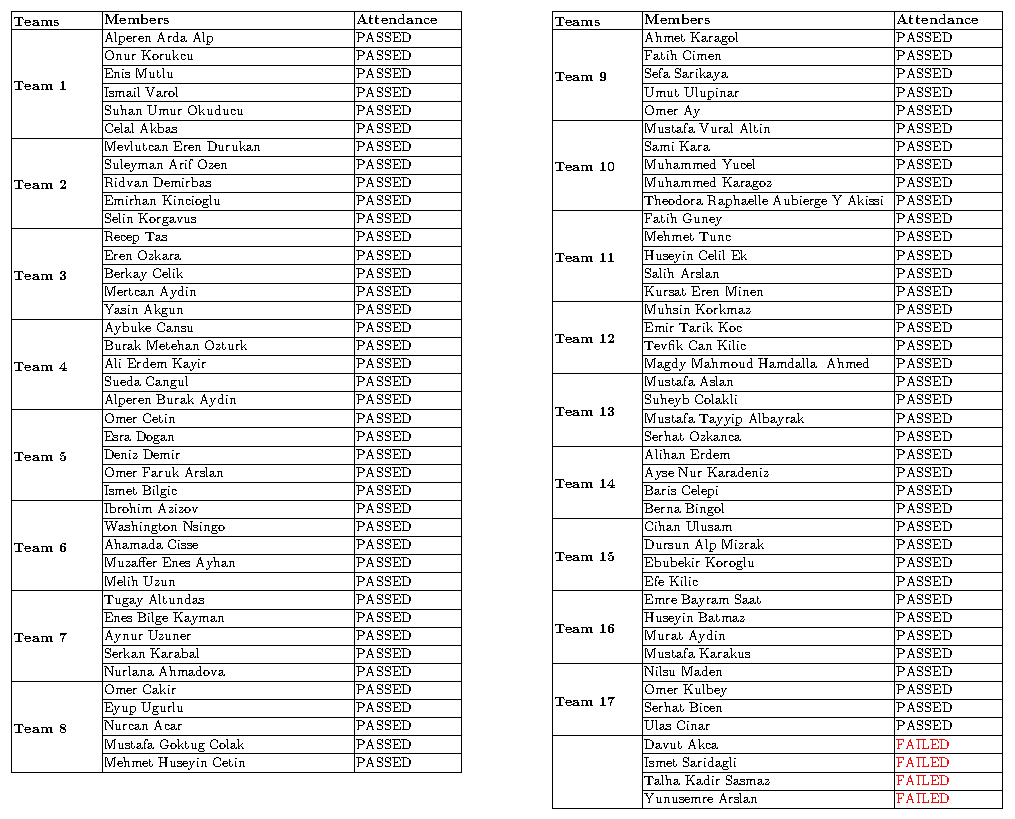
\includegraphics{teams.pdf}};
\end{tikzpicture}
\end{table}


\end{document}


